\documentclass{article}
  \parindent = 0mm % Sin sangría
  \usepackage[utf8]{inputenc}
  \usepackage[T1]{fontenc}
  \usepackage[spanish]{babel}
  \usepackage{graphicx}
  \usepackage{amstext}
  \usepackage{amsmath}
  \usepackage{booktabs}
  \usepackage{subfigure}
  \usepackage{footnote}
  \usepackage{hyperref}
  \usepackage{algpseudocode,algorithm,algorithmicx}
  \usepackage[font=small,labelfont=bf]{caption}

\begin{document}
  \begin{center}
    {\sc \large Enfoque de pulsos}
    
    {\sc \large Proyecto 2020}
    \linebreak

    {\rm Joaquín Correa - \today}
  \end{center}

  \section*{Introducción}

  Como proyecto de aplicación del algorítmo del Pulso propongo su aplicación al problema de ruteo de demanda y decisión de construcción de ciclovías en una ciudad, puede ser visto como una versión del problema de distribución de mercancías, sobre una red que puede ser mejorada mediante la construcción de instalaciones que mejoren la distribución. Utilizo el pulso como método alternativo a la programación matemática con el objetivo de escalar mejor en el tamaño de las instancias atacables, aunque con esto se pueda perder la exactitud de la solución, es decir lo utilizo como heurístca. Finalmente realizo un comparación en medida de lo posible con el MILP que resuelve el problema exacto e incluyo una sección con características propias y trabajo futuro.

  \section*{Problema}

  El problema consiste en decidir dónde construir ciclovías de manera que satisfaga las necesidades de los usuarios, representados por la demanda, de la mejor manera. Matemáticamente, el modelo consiste en un grafo dirigido y un conjunto de pares origen-destino donde para cada uno se tiene un valor de demanda (por ejemplo cantidad de personas). Para cada arco del grafo, se tiene un costo de usuario que corresponde al costo percibido por un usuario si lo utiliza para desplazarse y un costo de construcción de diversos tipos de ciclovías. Al construir una ciclovía sobre un arco, el costo de usuario disminuye. Finalmente se tiene un valor de presupuesto que limita la construcción de ciclovías.

  La formulación matemática es la siguiente:

  \begin{align}
    \text{min} & \sum_{k \in O} \sum_{i \in I} \sum_{e \in E} x_{ek}^i c_e^i & \label{eq:objective} \\
    \text{s.t.} & \sum_{i \in I}\sum_{e \in E_n^+} x_{ak}^i - \sum_{i \in I}\sum_{e \in E_n^-} x_{ak}^i = b_{nk} & \forall k \in O, n \in V \label{eq:flowconservation} \\
          & \sum_{i \in I} y_{e}^i \leq 1 & \forall e \in E \label{eq:onlyoneinfraactive} \\
          & \sum_{i \in I} \sum_{e \in E} m_e^i y_e^i \leq B & \label{eq:respectbudget} \\
          & x_{ek}^i \leq y_e^i  D_k & \forall e \in E, i \in I, k \in O \label{eq:restrictflowbyinfras} \\
          & x_{ek}^i \geq 0, y_e^i \in \{0,1\} &
  \end{align}

  Donde:
  \begin{description}
    \item[$O$]: Conjunto de pares origen-destino.
    \item[$I$]: Conjunto de infraestructuras.
    \item[$G=(V, E)$]: Grafo dirigido, compuesto por el conjunto de vértices $V$ y arcos $E$.
    \item[$c_e^i$]: Parámetro, costo de usuario de atravesar el arco $e$ utilizando la infraestructura $i$.
    \item[$b_{nk}$]: Parámetro, valor de la ecuación de conservación del flujo. Vale $D_k$ si $n$ es el origen de $k$, $-D_k$ si es el destino y cero en otro caso.
    \item[$m_e^i$]: Parámetro, costo de construcción de la infraestructura $i$ sobre el arco $e$.
    \item[$B$]: Parámetro, valor del presupuesto total de construcción.
    \item[$x_{ek}^i$]: Es la variable que modela el flujo de demanda del par origen-destino $k$, sobre el arco $e$ utilizando la infraestructura $i$.
    \item[$y_e^i$]: Es la variable binaria que indica si la infraestructura $i$ está activa en el arco $e$.
  \end{description}

  Y las ecuaciones:

  \begin{description}
    \item[(\ref{eq:objective})] Objetivo, se minimiza el costo total percibido por el flujo.
    \item[(\ref{eq:flowconservation})] Restricción de conservación del flujo.
    \item[(\ref{eq:onlyoneinfraactive})] Restricción que permite solo una infraestructura activa por arco.
    \item[(\ref{eq:respectbudget})] Restricción de presupuesto.
    \item[(\ref{eq:restrictflowbyinfras})] Restricción que permite al flujo utilizar la infraestructura activa únicamente.
  \end{description}

  \subsection*{Modelado}

  Se puede observar de la formulación, que si bien el grafo base es un grafo simple, se está trabajando sobre un multigrafo. Cada arco del grafo base es replicado tantas veces como cantidad de infraestructuras hay y cada replica tiene un costo de usuario y costo de construcción asociado.

  Lo que se busca son caminos óptimos por este multigrafo, con restricción de presupuesto, que determina para cada par de nodos, qué arco se elije, si se elije alguno. Notar que si se activa la infraestructura $i$ en el arco $e$, esta puede ser usada por cualquiera de los flujos entre pares origen-destino.

  Una cosa que no esta representada en el modelo, pero que se desprende de la realidad, es que siempre habrá una solución factible. Esto es debido a que se toma el grafo base como una de las infraestructuras cuyo costo de construcción es cero.

  \subsection*{Dificultades}

  Este problema, asi como fué formulado puede resolverse en un MILP solver para grafos no muy grandes de manera conveniente. Pero, al ser en parte un problema de programación entera sabemos es un problema contenido en $NP$ y por lo tanto, todavía, difícil de escalar.

  Particionando el problema en dos, con el solo objetivo de analizarlo, por un lado esta la decisión de cuál y dónde construir infraestructura y por otro la de encontrar el camino más corto para cada par origen-destino. La primera partición del problema es la difícil, la segunda, vista de manera aislada es un problema {\it fácil}: el flujo entre dos pares origen destino no esta relacionado con otros flujos, ni los arcos tienen capacidad. Por lo tanto, la segunda partición es simplemente el problema del camino mas corto entre dos puntos, repetido $card(O)$ veces. Lo que se busca en este trabajo, es utilizar el pulso para resolver ambos problemas al mismo tiempo.

  \section*{Aplicación del Pulso}

  Supongamos para simplificar, que tenemos un único par origen-destino. Debemos encontrar la asignación de infraestructuras a arcos que hagan mejor uso del presupuesto $B$. Si modelamos el grafo con infraestructuras como un multigrafo, esto se puede resolver como un problema de camino más corto con restricciónes o weighted-constrained shortest-path. Aquí es donde entra el algorítmo del Pulso.

  Es de suponer, que en la simplificación de un único par origen-destino, el pulso, o cualquier algorítmo exacto para el WCSP debe encontrar la mejor solución, la misma que encontraría el MILP solver. Ahora, si consideramos mas de un par origen-destino la cosa cambia.

  Si bien los pares origen-destino son independientes, la red subyacente es común, y el hecho de que una infraestructura esté activa o no en cierto arco puede determinar el camino mas corto entre varios pares origen-destino. Supongamos que se toma un par origen-destino y se ejecuta el pulso con cierta restricción de presupuesto. Luego se toma el siguiente par origen-destino y se ejecuta el pulso, con cierta restricción de presupuesto, si es que aún queda, y sobre el multigrafo luego de aplicar las infraestructuras que el pulso eligió para el primer par origen-destino. Se puede continuar este proceso iterativo hasta quedarse sin pares origen-destino. El hecho de quedarse sin presupuesto no afecta en lo mas mínimo, debido a que siempre habrán caminos cuyos costo de construcción sean cero. A grandes rasgos, este fue el camino que se siguió.

  Lo que queda por definir es la asignación de presupuesto para cada ejecución del pulso. Se decidió asignar a cada origen-destino la proporción de presupuesto relativa a la demanda de dicho par sobre el total, es decir: el presupuesto del par $k$ es $B_k = B  {D_k \over \sum_{s \in O} D_s}$.

  \subsection*{Consideraciones}

  Se implementó una versión del pulso simple que incluye las siguientes características:

  \begin{description}
    \item[Poda por costo]: {se corre inicialmente un Dijkstra sobre el reverso del grafo, para obtener una cota inferior del costo desde cada nodo al nodo objetivo. Luego se utiliza esta información para realizar la poda por costo.}
    \item[Poda por infactibilidad]: {se corre, para cada restricción, un dijkstra sobre el grafo reverso tomando dicha restricción como el costo. De esta forma obtenemos un valor mínimo de cada restricción requerido para llegar al nodo destino.}
    \item[Poda por dominancia]: {cuando un pulso llega a un nodo, se verifica que dicho pulso no esté dominado por algún otro pulso que ya se encuentre en el nodo.}
    \item[Cola de pulsos]: {En cada iteración, el pulso elegido es el que tiene menor costo proyectado. Es decir, cuyo costo actual mas la cota inferior del costo en el nodo, es menor.}
  \end{description}

  \subsection*{Modos de ejecución}

  El algoritmo requiere cuatro parámetros en su forma mas básica: el grafo, las restricciones y los nodos origen y destino. Se implementó de manera que sea mas bien un generador de caminos entre los nodos origen y destino. Para limitar la cantidad de caminos generados se puede puede incluir un parámetro que indica el costo máximo que deben tener los caminos generados y también existe la posibilidad de que devuelva unicamente el mejor. Estos últimos parámetros son de utilidad ya que la complejidad de buscar la mejor solución es mucho mayor que buscar una solución suficientemente buena, como se describirá en la sección de resultados.

  \subsection*{Otras opciones}

  \begin{description}
    \item[Descartar nodos mas lejanos]: Booleano, por defecto falso. Durante la ejecución del pulso, no considera nodos cuya cota mínima de costo sea mayor a la del pulso corriente. Esto puede ser deseado o no dependiendo del conjunto de datos.
    \item[Delta de descarte de nodos mas lejanos]: Numero, valor de la diferencia a prtir del cual se descartan nodos mas lejanos. También puede ser usado para forzar la elecciones de nodos mas cercanos, si se utiliza un valor negativo.
  \end{description}

  \section*{Casos de estudio}

  En esta sección se comparan los tiempos y las variables obtenidas de la ejecución del solver GLPK y el pulso. El pulso será ejecutado en varias configuraciones: $P_B$ será el pulso que busca la mejor solución y $P_S$ será el pulso donde se fuerza a encontrar una solución que sea tan buena como el costo del camino más corto sobre el grafo base multiplicado por $S$. Por ejemplo $P_{0.9}$ buscará soluciones que mejoren en un $10\%$ el costo del camino más corto.

  \subsection*{Ciudad Vieja}

  El primer nivel de comparación y ejecución del modelo se realizó con un grafo que representa aproximadamente\footnote{Se generó a partir de información de cruces de calles} el barrio Ciudad Vieja de Montevideo. En este grafo todas las calles van en ambas direcciones. Cuenta con 204 nodos y 734 arcos y su inexacta representación esta en la figura.

  \begin{figure}[]
    \centering
    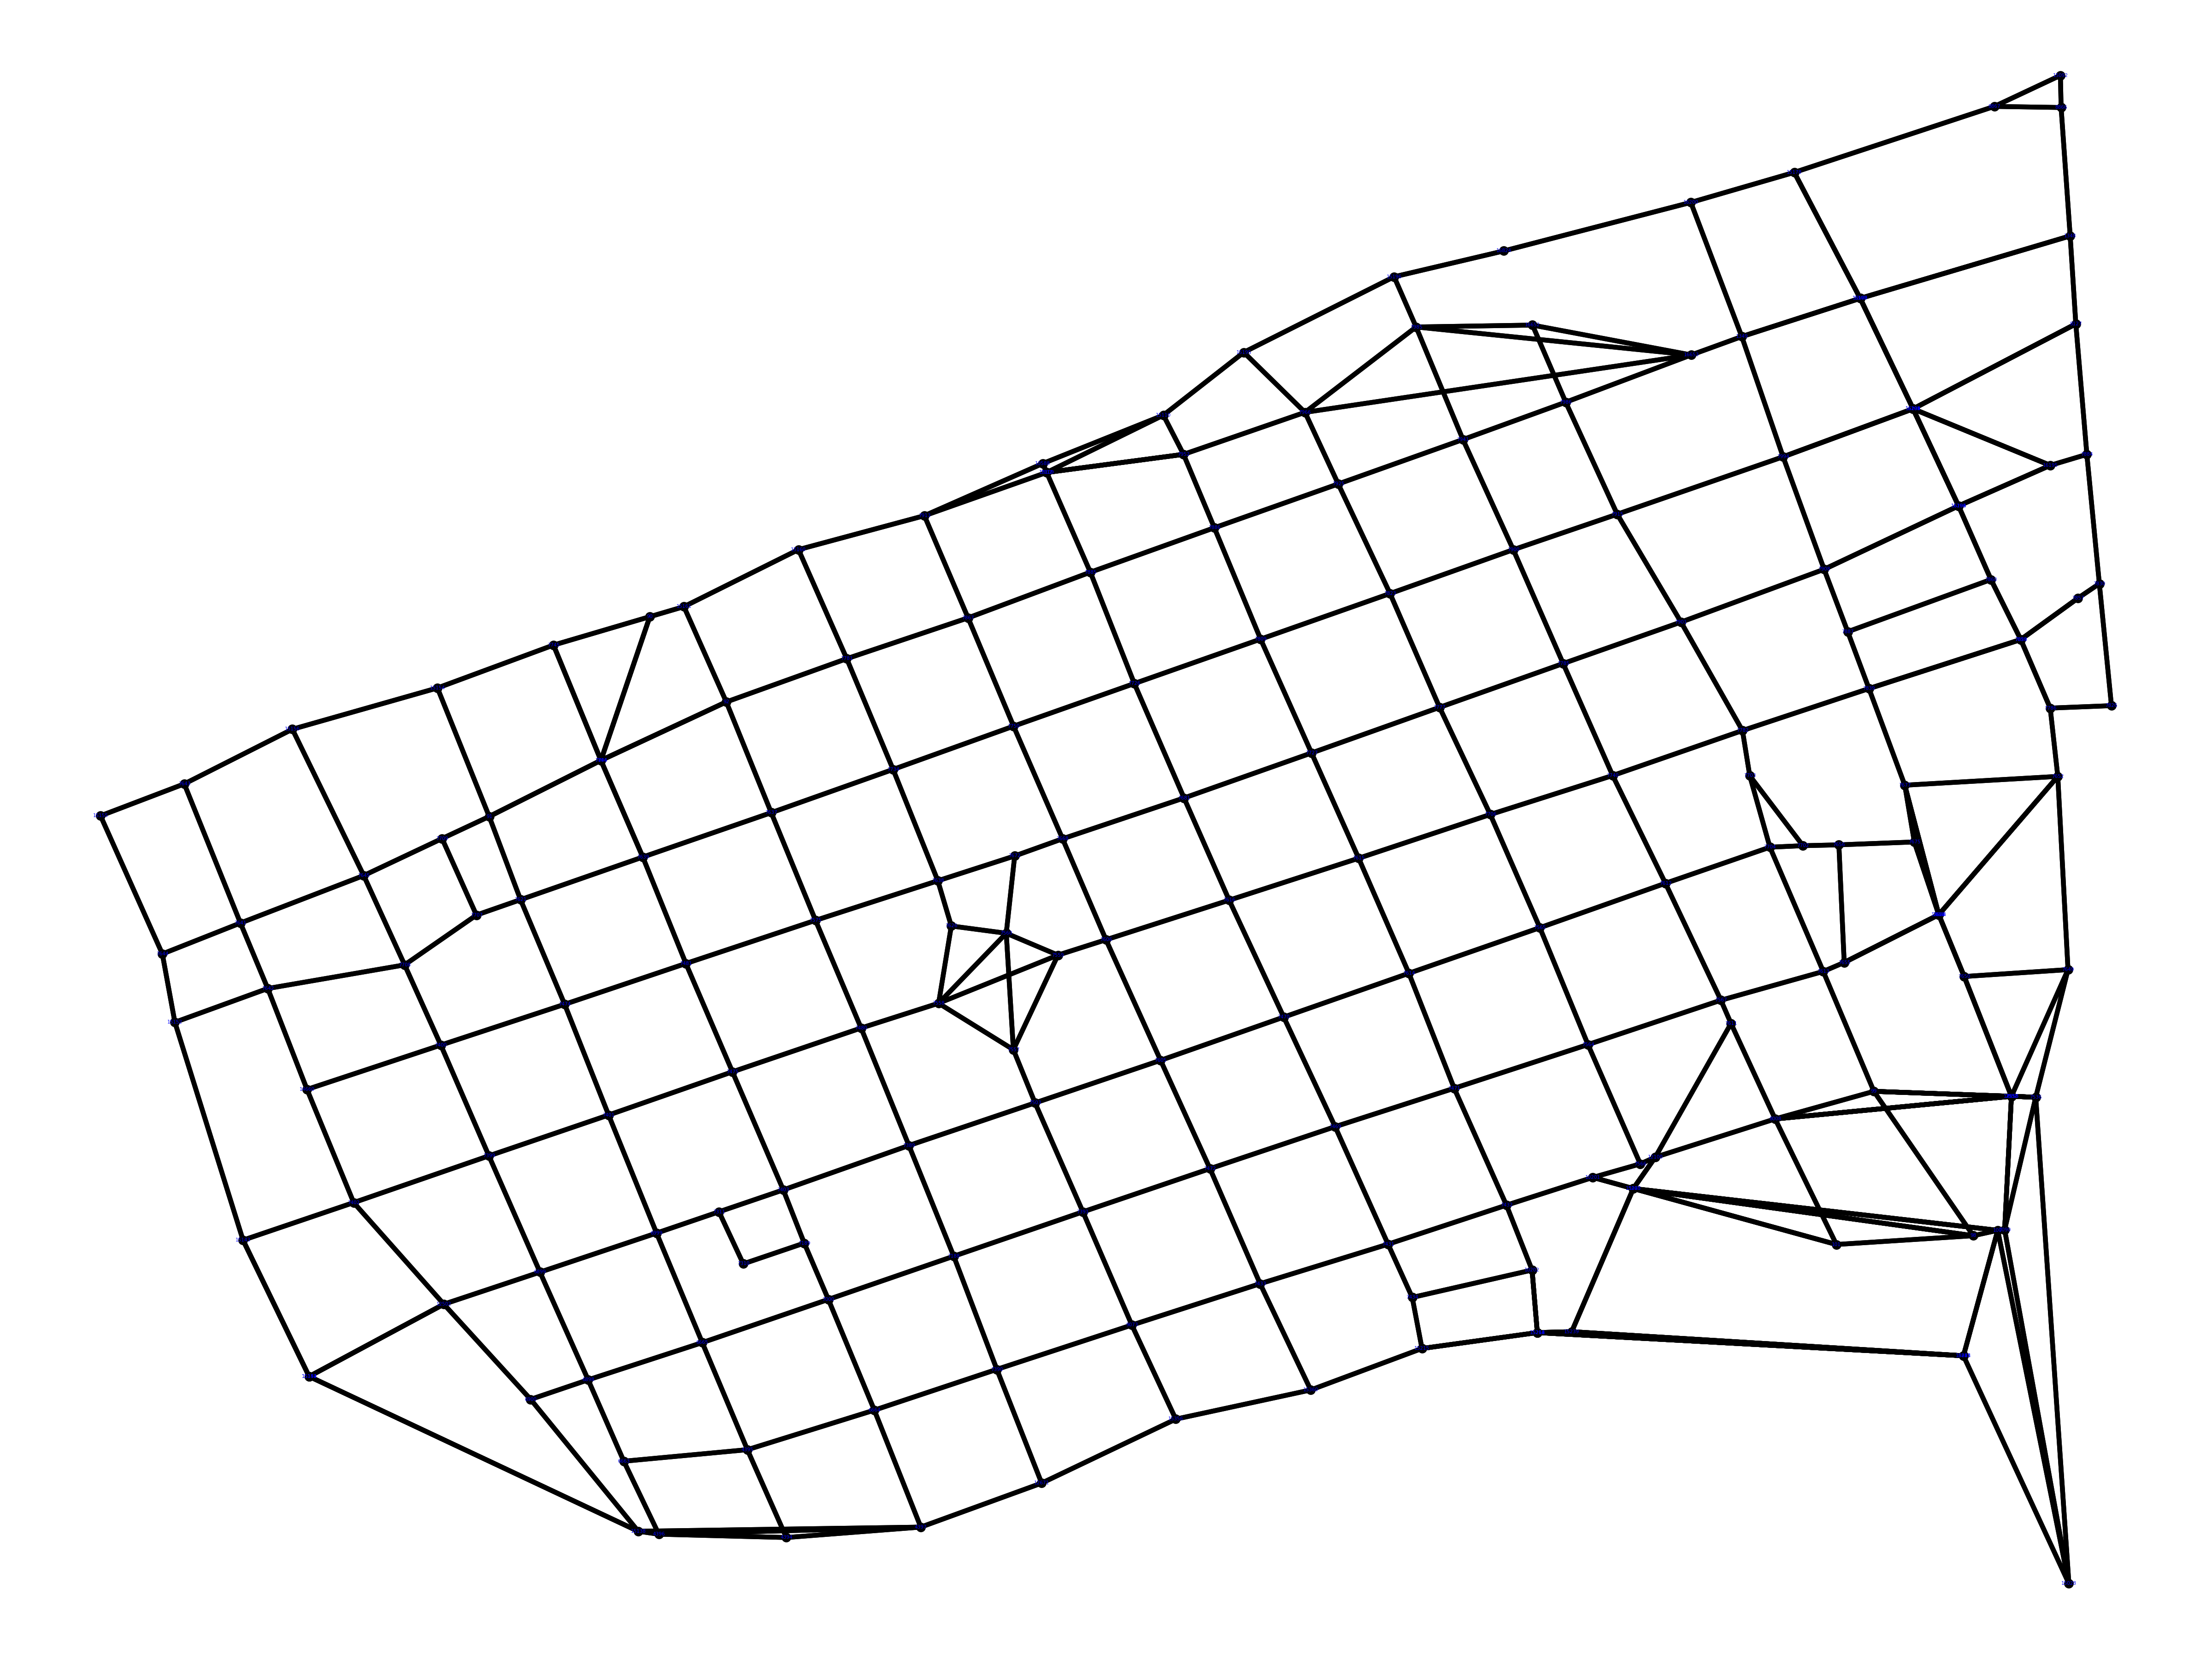
\includegraphics[width=6cm]{imgs/mdeo_med.png}
    \caption{Grafo de Ciudad Vieja}
    \label{ciudadvieja}
  \end{figure}

  Comparación de resultados.
  Comparar ejecución con glpk y cbc.

  \section*{Implementación}

  \section*{Trabajo futuro}

  \subsection*{Forzar mejores soluciones por par origen-destino}

  El parámetro para configurar la ganancia sobre el costo base por par origen-destino debería ser configurado para cada par. El problema con la forma de dividir el presupuesto es que pueden haber pares origen-destino con muy poca demanda relativa al total, que por lo tanto no logran un asignación de presupuesto que permita obtener la ganancia impuesta por el parámetro. Esto puede causar que no exista solución para algún par origen-destino, lo que causa un infructuso y largo tiempo de ejecución.

  \subsection*{Mejorar poda por costo}

  La poda por costo puede ser mejorada de de manera que se poden pulsos mas tempranamente. La poda actual solo considera la cota mínima del costo para obtener un costo mínimo proyectado hasta el destino. Sin embargo, este costo mínimo puede que sea inalcanzable debido a que los recursos que requiere no son factibles al sumarlos al pulso que se compara.

\end{document}
